\chapter{ Simulations and Results }\label{simulationsAndResults}

Recall that Liang-Wang example of a multimodial function:

\begin{equation}\label{againLiang}
f(x) = 
\sum_{i=1}^{20} \frac{\omega_i}{ \sigma_i \sqrt{2 \pi} } \exp \Big( -\frac{(x - \mu_i)^\tran (x - \mu_i)}{2 \sigma_i^2} \Big),	
\end{equation}
where $\sigma_1 = \dots = \sigma_{20} = 0.1$, $\omega_1 = \dots = \omega_{20} = 0.05 $ and the means $\mu_i$ are enlisted in Chapter \ref{motivation}.

Since we are dealing with stochastic simulations, do focus on the first two empirical moments analysis of different statistics in order to get some understanding of which \textsc{Swap Strategies} is better. 
Because of theoretical reasons mentioned in the Chapter \ref{theory}, one might be tempted to compare different \textsc{Swap Strategies} by considering the behaviour of their Колмогоров-Смирнов distance with the true underlying distribution, given by Eq. \ref{againLiang}. To this end the implemented KS statistics calculator was used, see Chapter \ref{KSimplementation}. The overall results are gathered in Figure \ref{KSdistancePlot}. 

The simulations involving the calculation of the \text{KS} statistics were carried out using the same parameters. The chains proposals have had their covariances matrix chosen so that about one in four proposal got accepted, which is the working rule-of-thumb among the practitioners of the stochastic simulation after the seminal work of \cite{ Roberts2001}. The covariances were chosen to be a slightly modified versions of those proposed by \cite{BaragattiLikelihoodFreeParallelTempering}.  Baragatti chosen the matrices to be of the form $T_i^2 \iii$, where $\iii$ is simply a 2 by 2 identity matrix and $T_i$ the $i^\text{th}$ temperature. The modification consisted in premultiplying the frist three matrices by $0.05$ and the last ones by $0.01$. The temperatures were also taken from baragatti and were equal to $T = (\,1,\, 2.8,\, 7.7,\, 21.6,\, 60\,)$. The computation involved 10000 iterations, a fourth of which was neglected being the burn-in period. The initial states were chosen from a uniform distribution on a square $[0,10]^2$ that contains all the means of the distributions that add up to form the considered mixture.


Figure \ref{KSdistancePlot} summarizes results of two different experiments consisting of different number of simulations --- the first of 40, the latter - of 120. There was no particular reason for choosing this amount of simulations --- the time-cost of the simulations that do calculate the KS statistics is however quite long and so we did not manage to collect information on the same number of simulations. The second group has larger standard deviation --- this can be attributed to differences in number of experiments. However what can be compared is the mean of these distributions. Also the standard deviation can be compared within the two groups. One can see that the differences in mean values of the KS statistics are small, possibly neglectable. However it remains a fact, that first three strategies give results that are on average smaller, so that they are closer to the original distibution in the KS sense. This is to say that generally the state-dependent strategies give better estimates than the state independent one, with the notable exception of the \ref{strat4}. One can also notice that the among the first three state-dependent strategies it is \ref{strat3} that has the lowest variance. Among the state independent stragies it also seems plausible not to draw swaps from a space restricted to only neighbouring ones, leaving it possible to exchange accepted proposals in the \textsc{Random Walk} phase between all the chains.   

\begin{figure}[ht]
	\centering 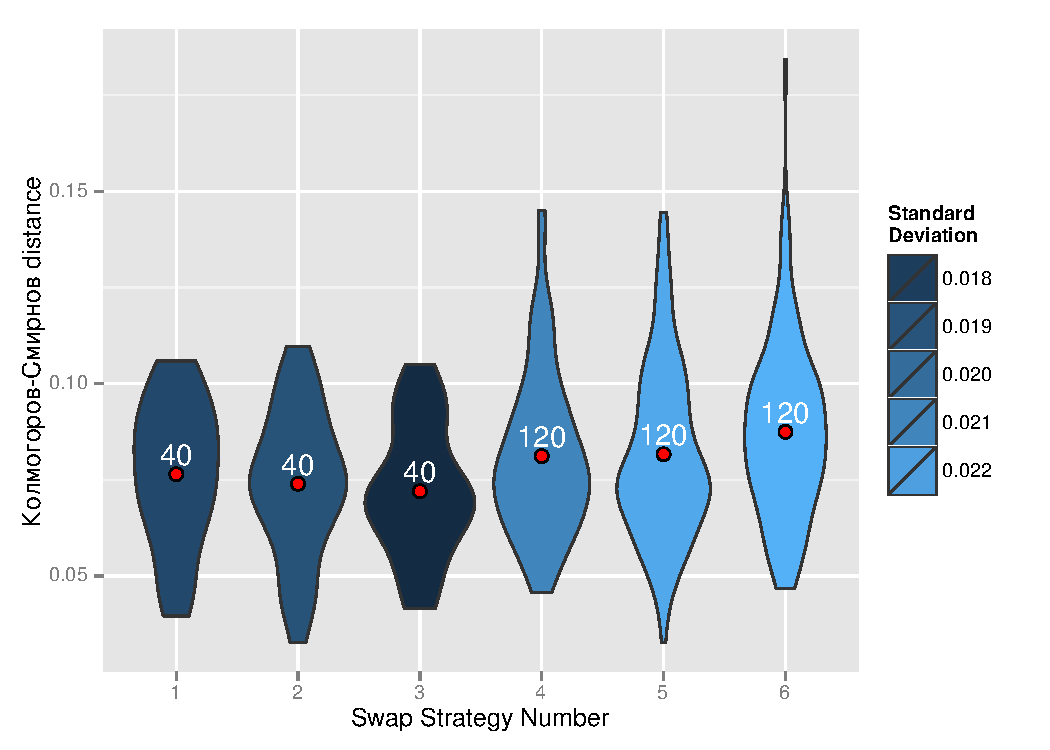
\includegraphics[width=\textwidth,keepaspectratio=TRUE]{./img/KSobs.pdf}
	\caption[Results of the KS-statistics simulations represented by a violin plot.]{Results of the KS-statistics simulations. The number of iterations a particular strategy was tested is annotated with the white numbers just above the red dots. The violin plots are simply smoothened empirical distributions. Red dots are their empirical means. The colour of the violin plots corresponds to the standard deviation, which is more instructive to study when considering subgroups with the same number of simulations.}\label{KSdistancePlot}
\end{figure}


\section{PTEEM as motivation for \textsc{Strategy I}}

One of the aims of the simualation was to compare ourselves with the results of \cite{BaragattiLikelihoodFreeParallelTempering}. In this article the author proposed an algorithm that supposingly combines the good sides of both the \PT\, and the Equi-Energy Sampler, orignally conceived by \cite{ Kuo2006}. The resulting algorithm, called PTEEM, again consists of two steps. In the original article it is assumed that the probability one faces is uniquely defined by a hamiltonian that describes the energy levels of a system, so that the density with respect to some measure $\lambda$ is
$$
	\pi(x) \propto \exp\Big(-h(x)\Big),
$$
however, as we shall see, it is not stringent a condition. The first phase is a simple random walk done independently for all the coordinate chains. The other step is more complicated. In PTEEM the \sspace\,is divided into regions called energy rings, being regions with the same energy levels, or simply $D_j = h^{-1}[H_j, H_{j+1})$, where $H_j$ are chosen {\it plus ou moins} heuristically. In the second phase of the algorithm two draws are perforem: (1) an energy ring is chosen at random among all those that contain at least two chains\footnote{One sets the number of energy rings and temperatures so that it is always the case.} and (2) two chains that are in the same energy ring are chosen at random and such proposal gets either accepted or rejected. 

The very idea of this approach is therefore much similar to what is being done in \ref{strat1} and comparisons with the results obtained there.      

In order to do so additional simulations were carried out without the evaluation of the \textsc{KS} statistics. The temperatures and proposal covariances were the same as those described above. We have reduced the overall number of iterations to 7500 with the burn-in period set to 2500 iterations as before. The initial states were drawn uniformly from a square $[0,1]^2$ for the reason of making it more difficult for the algorithm to reach all the modes.  

In Figure \ref{missingModes} one can notice that the choice of the starting point might have truly influenced the overall properties of the \PT. It plots the number of undiscovered modes for different strategies. What can be noticed is that all strategies sometimes fail to discover the modes that are far away from the starting points. The number of undiscovered modes is a measure of the algorithms mixing properties, as it says much about the algorithms inability to find itself in a certain place in the \sspace. 

To assign different sample points $\{ X^{[k]}\}_{k = 0}^\kk$ generated by the algorithm to particular modes a classifier had to be constructed. In our case, a randomised $\chi^2$-classifier was used. The reason behind it is that if a random vector is normally distributed and centered at point $x$, then the distance from mode $x$ is $\chi^2$-distributed. So, one can assign a given point to its mode at random in the following way: for one sample point (1) calculate the probabilities of observing radius bigger than the one observed for all the modes and (2) chose at random the mode with the probability proportionate to the quantities calculated in point (1). Such a procedure assures that points that are closer to a particular mode are much more likely to be assigned to it. Also, if there are sevaral points in the proximity of two modes, then the randomness allows to redistribute the points in a way that does take into account that some of the probability mass comes from one mode, and some from the other.   

Studying Figure \ref{missingModes} one notices easily, that all the state-dependent strategies have a clear advantage over the state-independent strategies in their ability to explore most of the \sspace. Above all, \ref{strat6}, where only neighbouring chains are permitted to exchange accepted proposals from the \textsc{Random Walk} phase, fails miserably and in 5 promiles of cases does not even  discover the closest modes to the place of initial drawing. It is \ref{strat3} that managed to discover most of modes most frequently and always discovers all the nearby modes to tha place of initial drawing. We think that this is also the reason why \ref{strat3} scores better in the KS tests, however it remains obscure why \ref{strat4} acts similarly to state-independent strategies when it is quite good at exploring most of the \sspace. 

\begin{figure}[ht]
	\centering 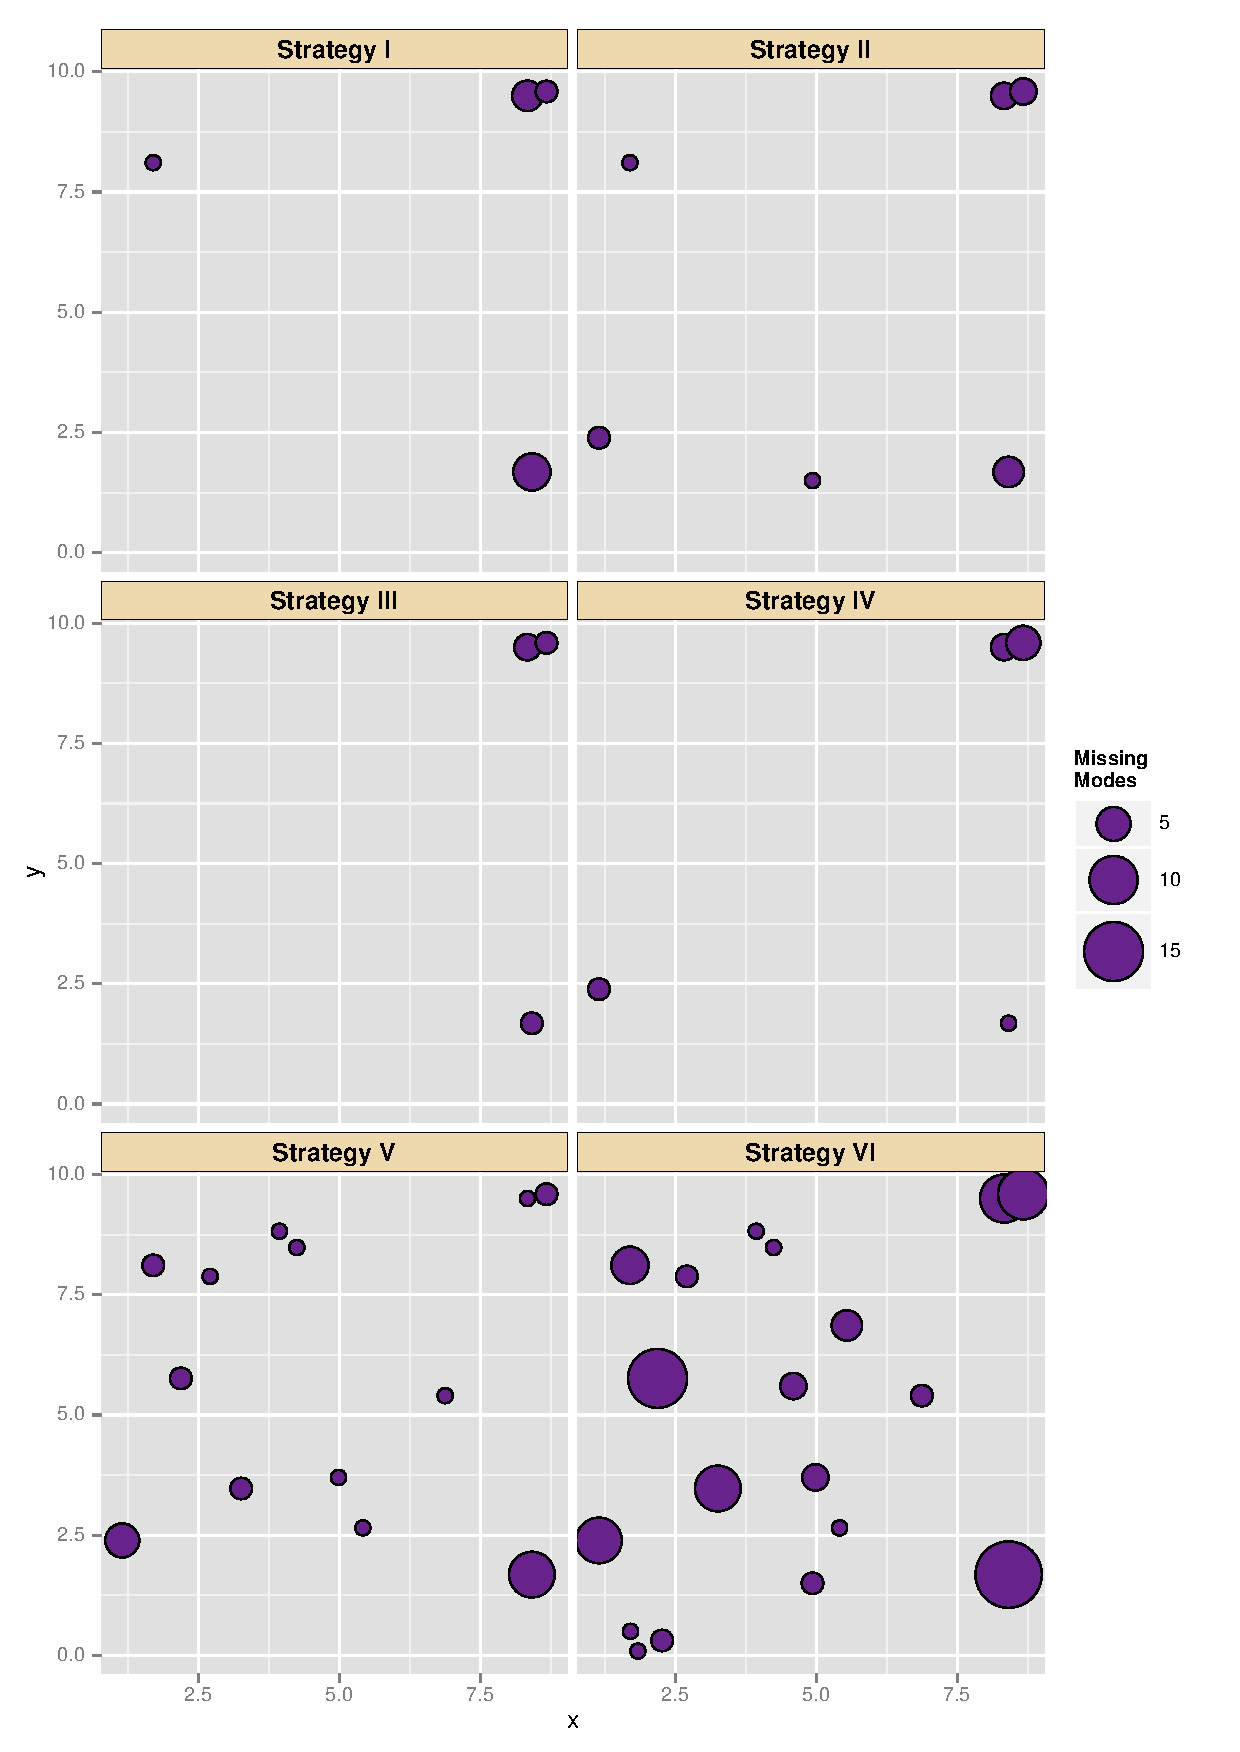
\includegraphics[height=.7\textheight,keepaspectratio=TRUE]{./img/ggplotMissingModes.pdf}
	\caption[Undiscovered Modes by the \PT\,representented by a baloon-plot.]{
		The baloon plot depicts the failure of the \PT\, under different swapping regimes to discover during one simulation all the components of the Liang's disribution, defined by Eq. \ref{againLiang}. The sample points from the simulated chains were assigned to modes using the randomised $\chi^2$-classifier. The size of the baloon corresponds to the number of simulations, out of 1000, that resulted in not assigning any points to the particular mode. The less dots appear on the plot, the more more modes were discovered, 
	}\label{missingModes}
\end{figure}

Another way of comparing different strategies is to see how they manage to approximate the weights of different modes in the entire distribution. A possible criterion for measuring the quality of approximation is to look upon the average absolute error. It averages the absolute distance of a simulation approximation of weight from the true one, equal to $0.05$. Figure \ref{AAE} summarises the results of such procedure.

What can be seen in Figure \ref{AAE} is that again the state-independent proceduters are notably worse in prescribing the correct weights to different modes. The average absolute errors reach $0.025$ and even $0.03$ which amounts to respectively $50\%$ and $60\%$ of the true value, which is much. It's worth stressing however that even the winning \ref{strat1}, that manages to score best in 18 out of 20 modes, sometimes reaches a $50\%$ relative\footnote{Again with respect to $0.05$} error. It's best result is to score a mearly $30\%$ relative error.         

\begin{figure}[ht]
	\centering 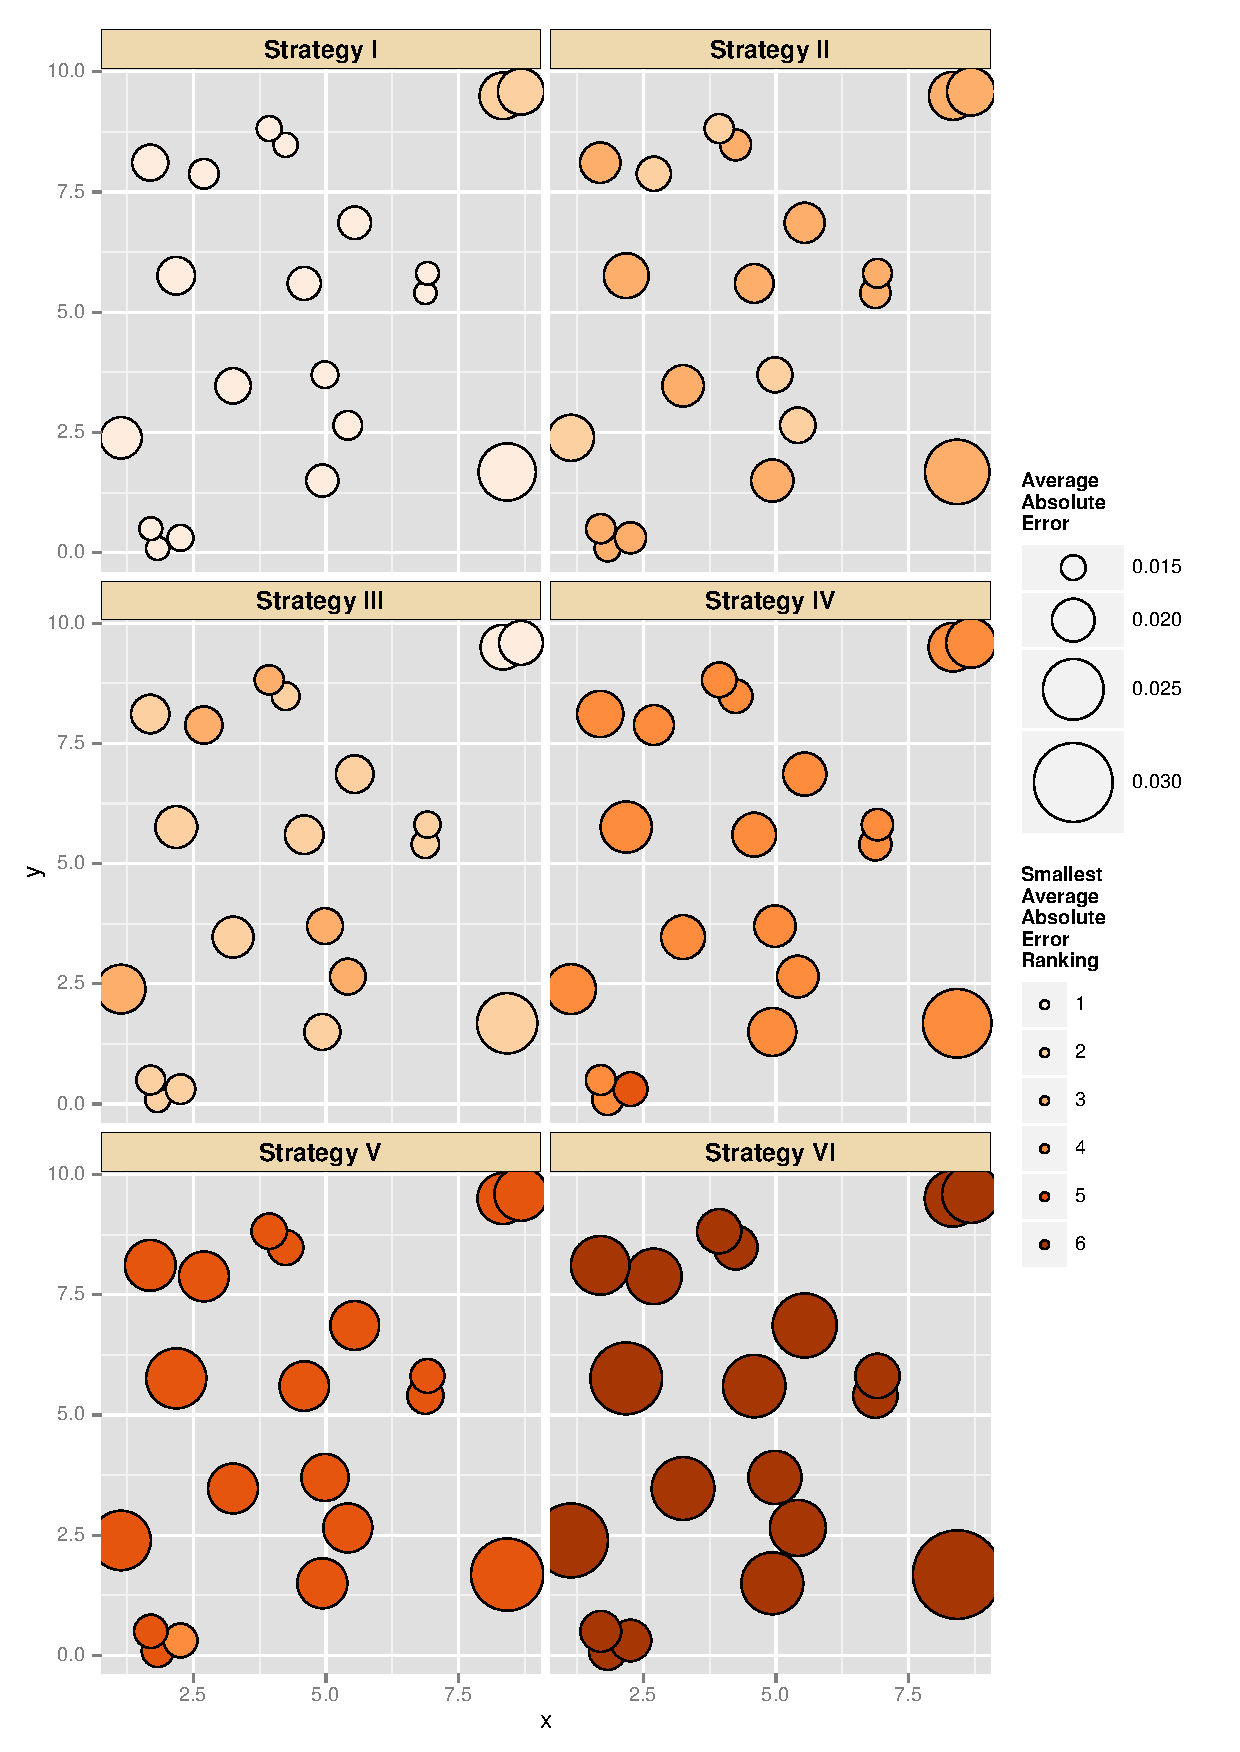
\includegraphics[height=.7\textheight,keepaspectratio=TRUE]{./img/ggplotAverageAbsoluteError.pdf}
	\caption[Average Absolute Errors in simulations consisting of 2500 iterations of the \PT.]{
		The baloon plots depicts the errors of the \PT\, in evaluating the weights of different components of the Liang's mixture, defined by Eq. \ref{againLiang}, under different Swap Strategies. The sample points from the simulated chains were assigned to modes using the randomised $\chi^2$-classifier. The error is calculated simply as the $l^1$ distance of results divided by the number of observations, being equal to 1000. It is being calculated seperately for different strategies and different distributions that compose the mixture; all of them appear with weight being equal to 0.05. The dots are coloured according to their position in the overall ranking of errors, done separately for every mode of Liang's distribution, so that the darker they are, the bigger was the error for a particular mode. The sample points from the simulated chains were assigned to modes using the randomised $\chi^2$-classifier.   
	}\label{AAE}
\end{figure}

One can also wonder whether the quality of estimates improves whith longer runs of the algorithm, that is, whether the procedure is stable and convergent. Figure \ref{shortAndLongSimulations} gives an answer to such question. All the rhombi that correspond to longer runs of the algorithm are found inside the dots that represent the shorter ones --- significantly longer runs (in the above example three times longer) do lead to overall improvement in the precision of estimates. This improvement amount to about a 50\% reduction in error, which stems from visual inspection of the length of rhombi's diagonal wiht respect to the dots' diameter. One notices also slight reshufflements in ranking among the state-dependent strategies, as in different plots pairs dot-rhombus with different colour schemes appear: \ref{strat3} seems to overtake \ref{strat2} in ranking. One can also obeserve that among the state-independent strategies there no difference in rankings, \ref{strat6} restricted to swaps between neighbouring chains loosing with \ref{strat5}. One can also notice that \ref{strat4} has better results than \ref{strat5} in one additional mode. 

\begin{figure}[ht]
	\centering 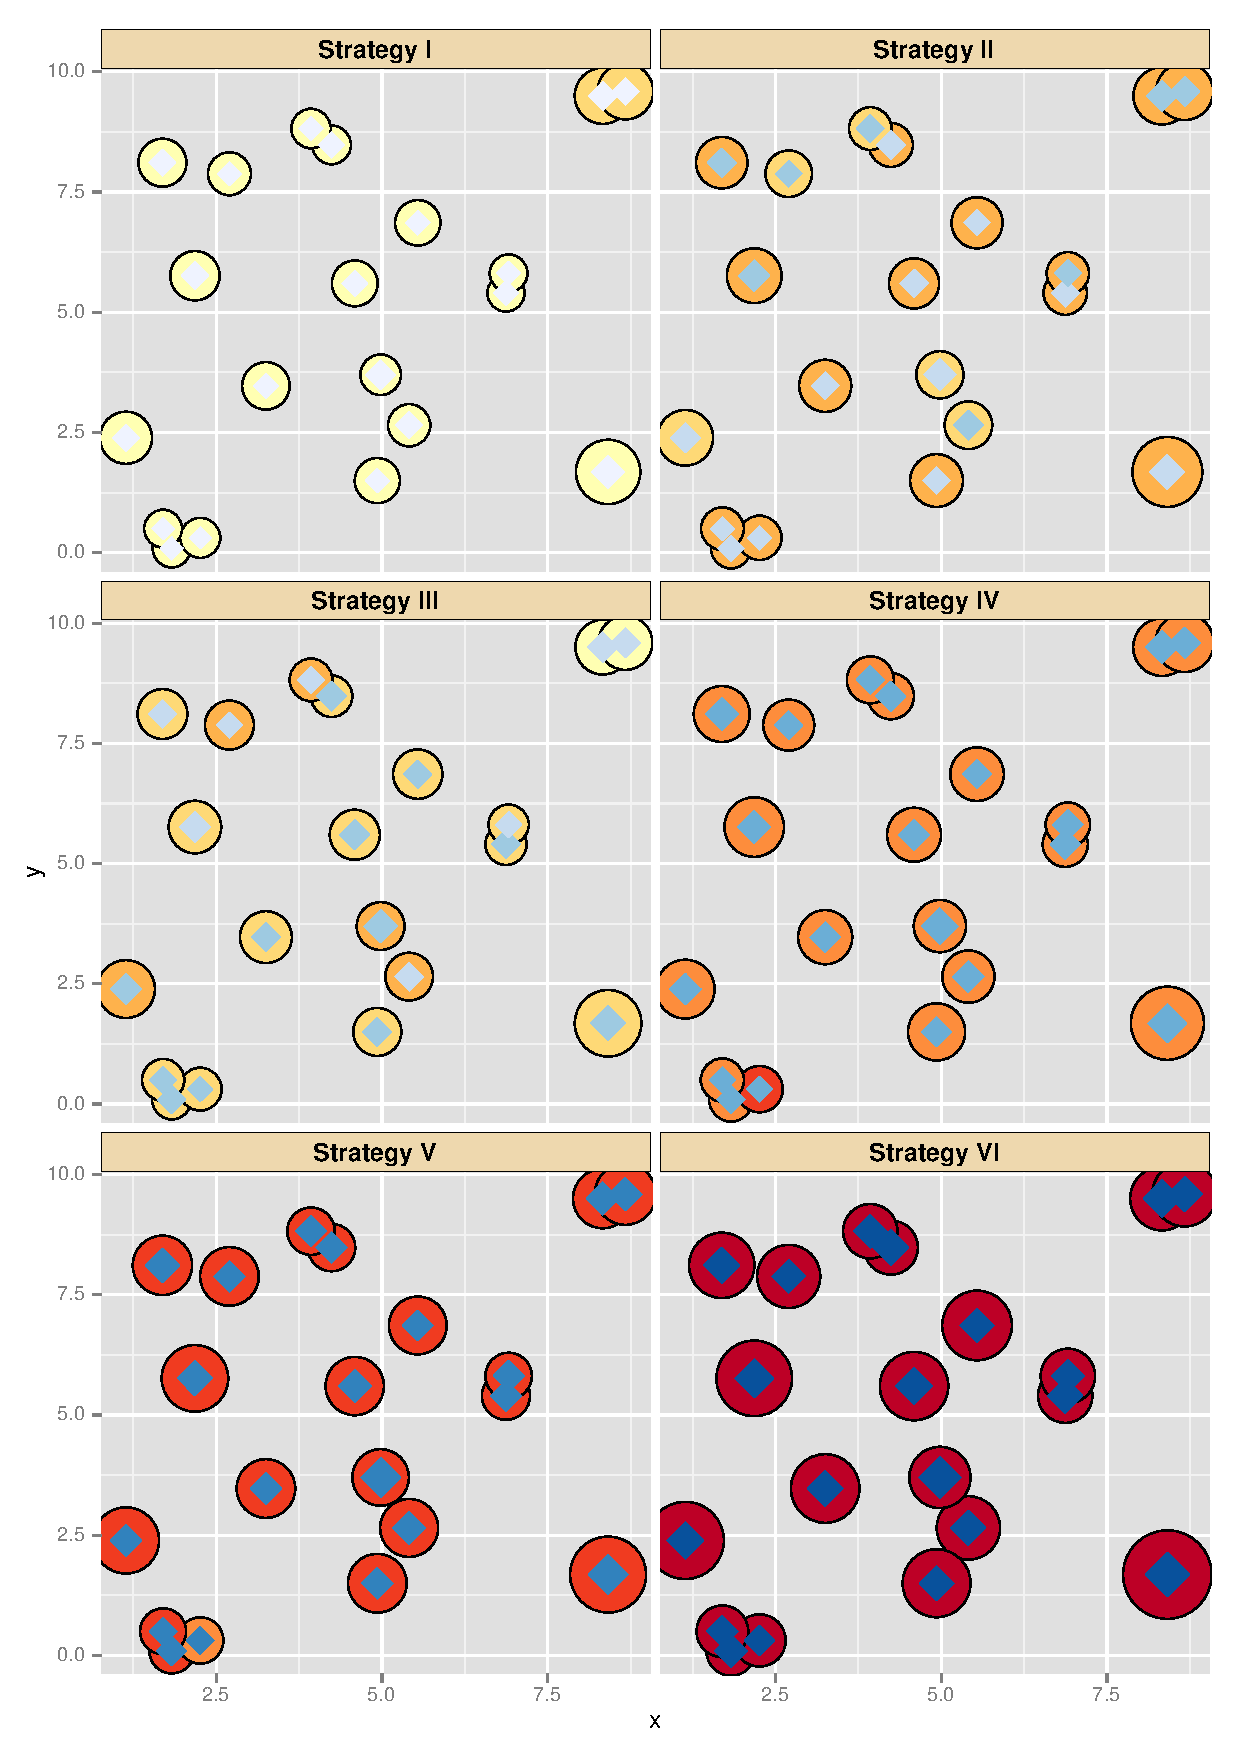
\includegraphics[height=.7\textheight,keepaspectratio=TRUE]{./img/bigSimulationOverlayed.pdf}
	\caption[Average Absolute Errors comparison between 2500 and 7500 iteration-long runs of the \PT.]{
		This figure explores the differences in the quality of the estimations of modes between shorter and longer runs of the \PT\, for different swapping strategies. Both dots and rhombi represent the Average Absolute Errors: dots correspond to shorter simulations --- 2500 iterations, and rhombi to longer simulation --- 7500 iterations, {\it ceteris paribus}. If the vertices of a given rhombus were to touch the border of a dot then errors would be the same; this, however, never occurs and the estimates are indeed much sharper. Again the colours intensity helps distinguish among the ranking of approximation: lighter colours correspond to smaller values of errors. 
	}\label{shortAndLongSimulations}
\end{figure}




One can also try to compare different strategies in their task of actually appoximating different integrals. We have restricted ourselves to evaluate how the algorithms handle the task of actually calculating the real moment of Liang's distribution. These are readily computable analytically. 

In Figure \ref{momentsBaragatti} we compare the outcomes of different Swapping Strategies in this particular task. Observe that all the strategies on average perform admiringly in this task, since the average empirical estimate of moments is very near the true value --- the rhombi are usually near the centre of the dot that marks the true value. One can see that all the algorithms better estimate the first coordinate of the mean than the second. Also the estimates of the covariance matrix show, that the variance of the $y$ coordinate have bigger variance. Within the state-independent group of strategies it is also apparent that the possibility to accept swaps from not-neighbouring chains results in a concentration of the empirical distribution. However results of state-dependent strategies seem to be fairly comparable. 

\begin{figure}
	\begin{minipage}[b]{.5\linewidth}
		\centering 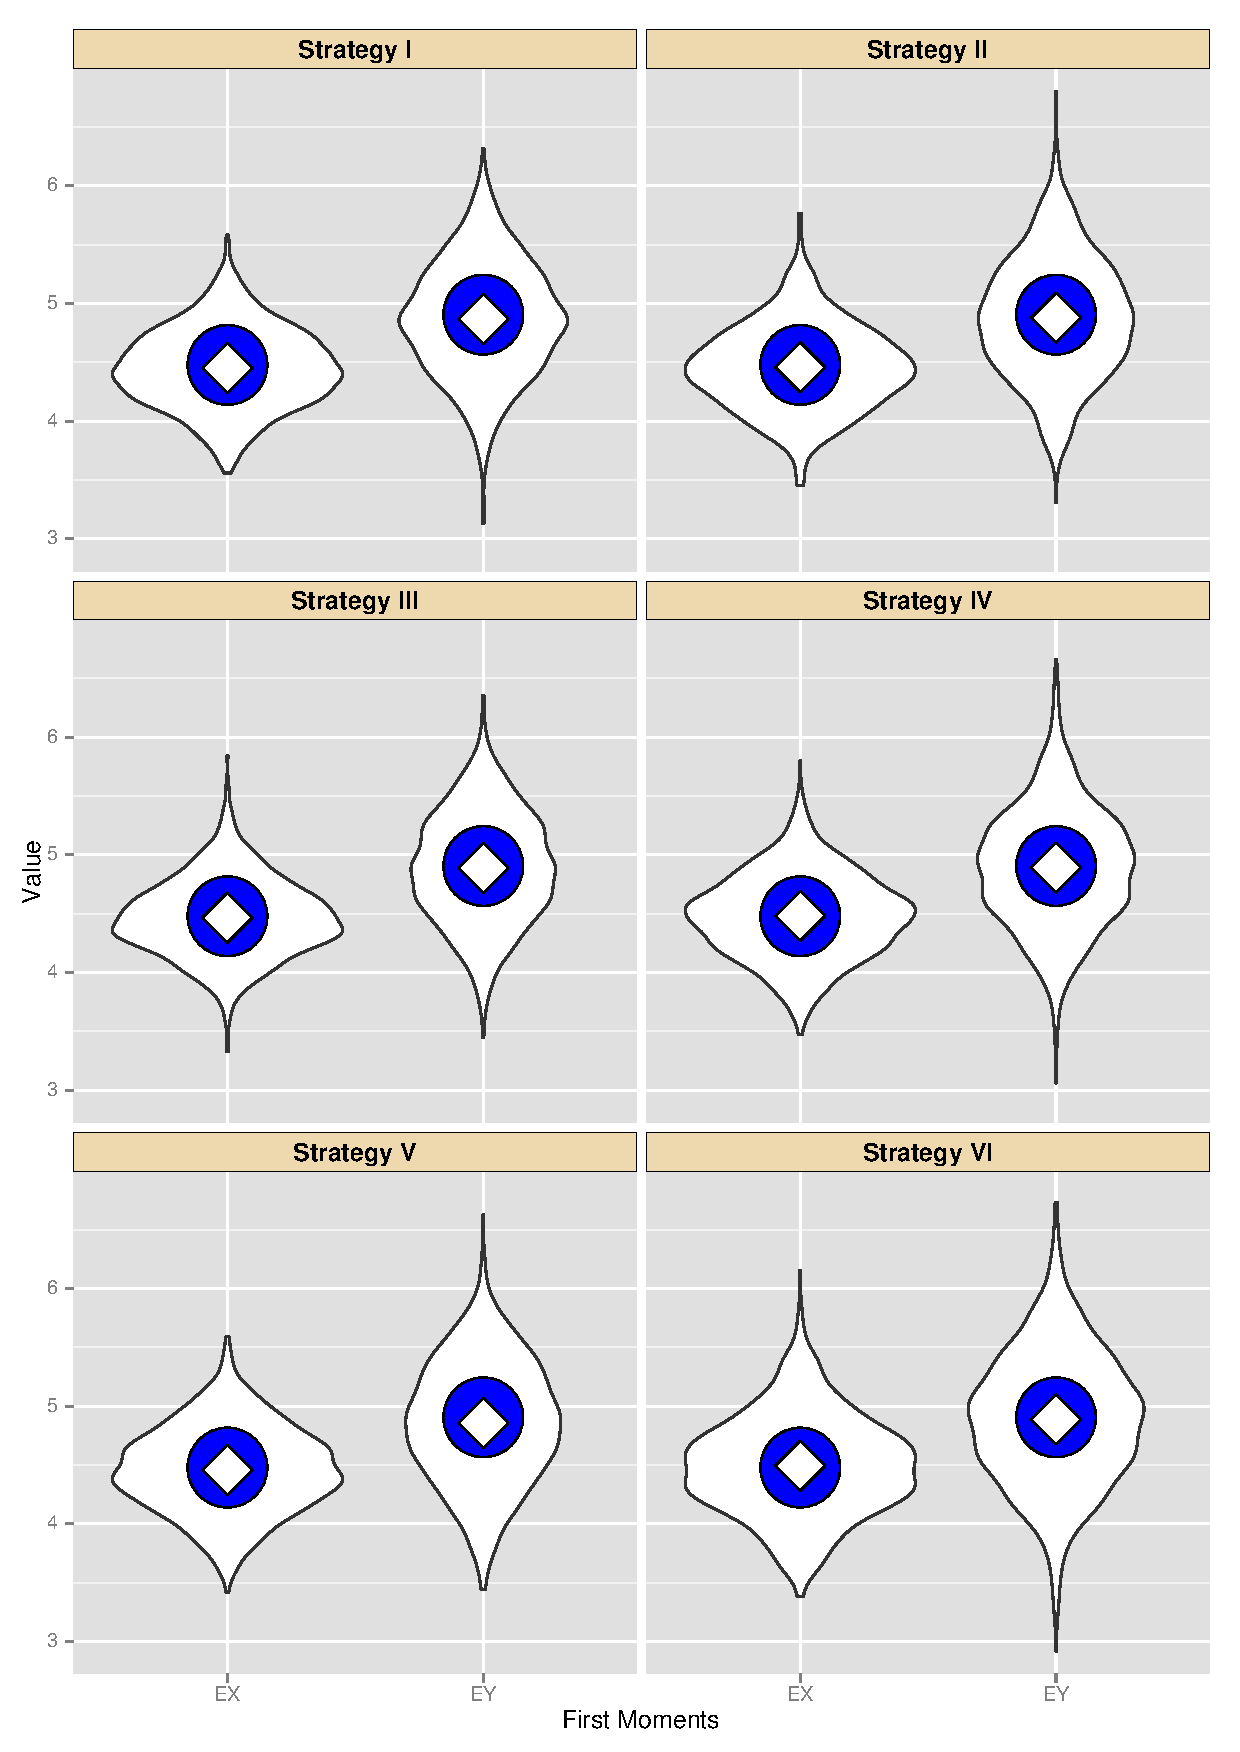
\includegraphics[width=\textwidth,keepaspectratio=TRUE]{./img/firstMomentsBaragatti.pdf}
		\subcaption{First Moments}\label{firstMomentsBaragatti}
	\end{minipage}%
	\begin{minipage}[b]{.5\linewidth}
		\centering 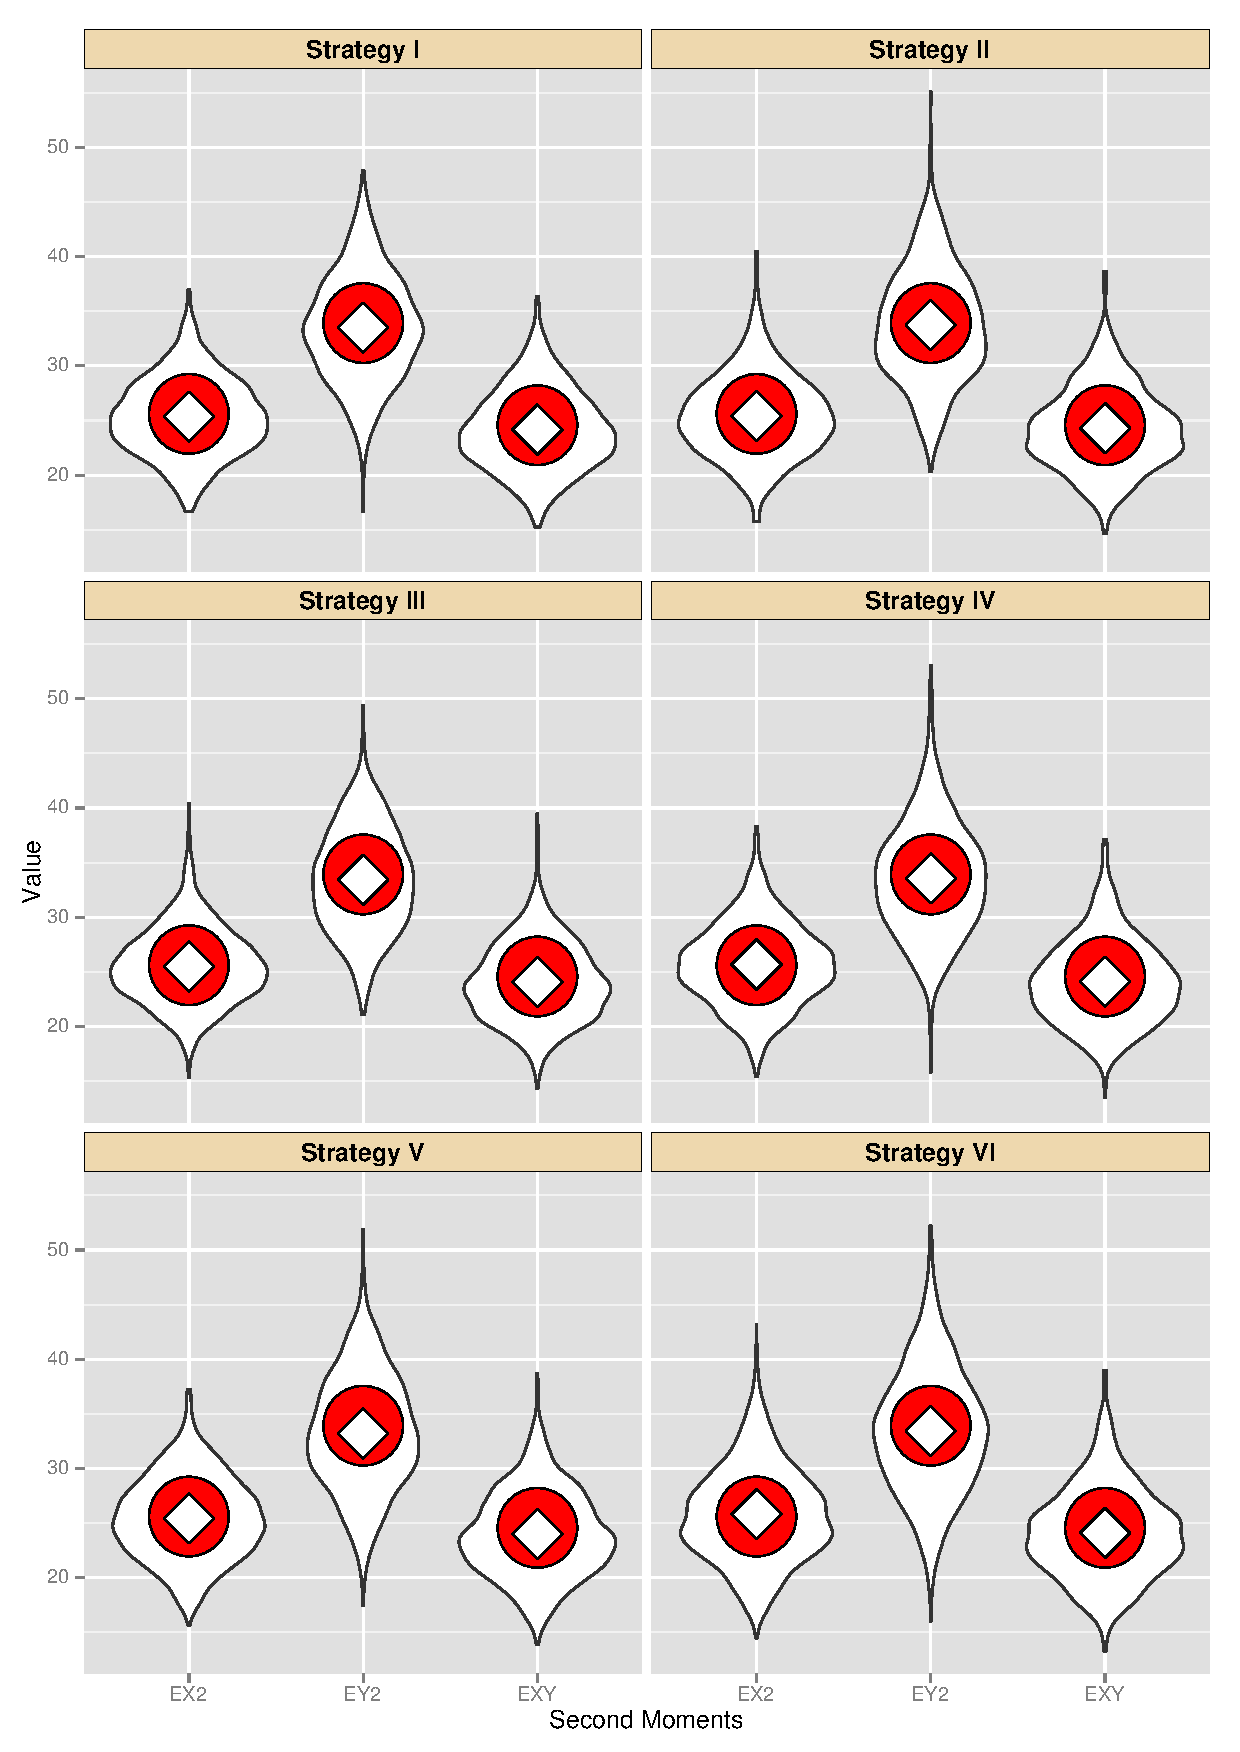
\includegraphics[width=\textwidth,keepaspectratio=TRUE]{./img/secondMomentsBaragatti.pdf}
	\subcaption{Second Moments}\label{secondMomentsBaragatti}
	\end{minipage}
	\caption[First and Second moments of the Liang Distribution approximations --- distributions represented by a violin-plot.]{
		The violin plots depict smoothened distributions of first and second moments of the Liang mixture, described by Eq. \ref{againLiang}, for different \textsc{Swap Strategies}. The empirical means are ploted as white rhombi on the blue background. The blue dots are centered at Liang Distribution's exactly calculated moments, so that one can asses the differences of theory and experiment simply by comparing the relative posititioning of the centres of rhombi and dots.
	}\label{momentsBaragatti}
\end{figure}
